\documentclass[letterpaper,12pt]{article}
\usepackage{utr}
\usepackage{hyperref}
\usepackage{courier}
\usepackage{longtable}
\usepackage{textcomp}
\usepackage{graphicx}
\usepackage{tabulary}
\usepackage{tabularx}
\usepackage{amsmath}
\usepackage{float}
\usepackage{wrapfig}
\usepackage{enumitem}
\usepackage{chngpage}
\usepackage[margin=1in]{geometry}
\usepackage{graphicx}
\usepackage{listings}
\usepackage{setspace}
% \usepackage[T1]{fontenc}
\lstloadlanguages{C++,Pascal} %Pascal for Unicon syntax
%\usepackage[all]{xy}
\lstset{language=C++}

\title{Pattern Matching in Unicon}
\author{Clinton Jeffery, Sudarshan Gaikaiwari and John Goettsche}
\trnumber{18b}
\date{\today}

\newcommand{\squeezeup}{\vspace{-1em}}
\begin{document}

%\begin{samepage}

\abstract{
  Unicon Version 13 introduces a pattern type for matching strings.
  The literal constants for this pattern type are strings, csets, and
  regular expressions, while the operators and composition features
  are based on the SNOBOL4 pattern type.
  Patterns are both an alternative and an addition to the string
  scanning control structure.
  }

\maketitle

%\end{samepage}

\section{Introduction}

This technical report is a user's guide and reference to the pattern
data type in the Unicon programming language. In order to understand
this report, it will be helpful if the reader is familiar with Icon
and Unicon's string scanning control structure. Compared with
traditional methods, the pattern type allows more concise, more
readable, and/or faster solutions for many string analysis problems.
It is especially useful when:

\begin{itemize}
\item the format of strings is less than ideally structured
\item the complexity of the patterns to be matched is high
\item the ability to compose new patterns on the fly at runtime is
desired
\item there is a lot of string data and performance may be important
\end{itemize}

\subsection{Icon Scanning vs. Snobol Patterns vs. Unicon Patterns}

Icon replaced SNOBOL's pattern data type with a
string scanning control structure.  The pattern type reintroduced
into Unicon Version 13 is important for all the reasons that data
is more convenient to manipulate than code: easier composition and
reuse, modification and dynamic altering of patterns on the fly, and
so on. SNOBOL veterans have complained that the Icon string
scanning control structure is not as concise as SNOBOL patterns.
Unicon patterns answer that criticism.

A ``hello, world'' type of example is

\begin{verbatim}
procedure main()
   write(read() ?? <[hH]ello[ \t]*[wW]orld>)
end
\end{verbatim}

This program reads a single line from standard input and executes a
pattern match. The pattern will match as long as ``hello'' is followed
by ``world'', with optional whitespace in between. Either or both
words may be capitalized. If the match is successful, the substring
that matched is written to standard output, stripped of any leading
or trailing characters.

\subsection{The Two Types of SNOBOL Pattern Statements}

The two types of SNOBOL pattern statements, pattern matching and
pattern replacement, use the following two templates:

\begin{verbatim}
label subject pattern goto
label subject pattern = object goto
\end{verbatim}

Instead of using a ``label'' or ``goto'', the pattern match in Unicon
is a predicate expression, often used as the condition in an \texttt{if}
expression.  The SNOBOL pattern replacement statement has a more
interesting Unicon embodiment.  If a pattern match is performed on a
variable, the matched portion is a substring variable that may be
assigned with a replacement string.  The following example searches
for (a subset of) American-style dates and replaces them, moving the
day to the beginning, as is common in other countries.

\begin{verbatim}
procedure main()
   s := "Adam's birthday is February 28, 1969. He is no spring chicken."
   month := <January|February|March>
   day := <[1-3]?[0-9]>
   year := <[0-9]{4}>
   s ?? month->part1 ||" "|| day->part2 || (", "||year)->part3 :=
      part2 || " " || part1 || part3
   write(s)
end
\end{verbatim}

This is neither SNOBOL nor Icon, exactly.  Details of the patterns and
operators used are presented later in this report. After you have read
about them, as an exercise you can modify the regular expressions here to
be more complete or more correct.


\section{Pattern Matching Foundations}

Pattern matching consists of two phases: (1) construction of a
pattern to be matched, and (2) application of the pattern in a context.
Application of a pattern in turn features two primary modes: match
and search. A match reports whether a pattern matches a given string
at a specific location.  Its result is an extent of the match, or a
failure. The search for a pattern involves finding a match, reporting
the start position and perhaps extent where the match has occurred.

In string scanning, the duality of match and search is seen in the
built-in function set: {\tt find()} is a search for a {\tt match()};
{\tt upto()} is a search for an {\tt any()}. Pattern matching has
two forms of pattern
application: anchored and unanchored. An anchored pattern match tests
whether a pattern occurs at a given position within a given subject
string. An anchored match is performed by the tabmatch operator {\tt =p}.
It is legal only within a string scanning environment.

\begin{verbatim}
s ? { ... =p ... }
\end{verbatim}

An unanchored pattern match is a search for a match, performed with
the syntax

\begin{verbatim}
s ?? p
\end{verbatim}

\noindent This is a new string scan in a new environment, except with
a pattern to match instead of an expression on the right side.


\section{Pattern Literals}

The simplest to interpret pattern values are literals, expressed as
{\em regular expressions\/}. Regular expressions are concise, simple,
readable, and sufficient for many purposes.
However, regular expressions cannot match
everything. Additional, more complex patterns can be constructed using
{\em pattern constructor\/} operators and functions, described in the
next section.

Unicon regular expressions consist of a regular expression body,
enclosed in less than ({\tt $<$}) and greater than marks ({\tt $>$}),
as in the example

\begin{verbatim}
   x := <abc>
\end{verbatim}

A regular expression is a pattern constructor that produces a single
result of type pattern that may be used in subsequent pattern
construction and matching operations.  Within the body of a regular
expression, most printable characters match themselves, and normal
Unicon variables, values, operators and syntax constructs do not have
their usual meaning. Instead, the following operators are supported:

\begin{description}
\item [ordinary characters evaluate to themselves] -- for example
${\tt <a>}$ is a pattern that matches the letter {\tt a}.  Spaces
inside a regular expression literal are not typically significant;
to allow a space as part of a pattern it must be quoted.
\item [implicit concatenation] -- inside a regular expression,
juxtaposing two symbols is a concatenation. $<abc>$ matches the
string abc.
\item [strings evaluate to their contents] -- for example,
${\tt <}${\ttfamily"}${\tt abc}${\ttfamily"}$>$ and ${\tt <abc>}$
construct the same
pattern. Such ordinary Unicon string literals are the way to match any
character that would otherwise be interpreted as a regular
expression operator.
\item [alternation] -- the lowest precedence regular expression
operator is alternation, indicated by a single vertical bar, which
means either-or. ${\tt <a\vert b>}$ matches either {\tt a} or {\tt b}.
Alternation is lower precedence than concatenation.
\item [Kleene star] -- a unary suffix asterisk indicates that a
pattern may occur zero or more times. Kleene star is of high
precedence, so {\tt $<abc*>$} matches {\tt a} followed by {\tt b}
followed by zero or more {\tt c}'s. In contrast, {\tt $<(abc)*>$}
matches zero or more repetitions of {\tt abc}, and {\tt $<[abc]*>$}
matches zero or more occurrences of a, b, or c in any order.
\item [csets] -- within regular expressions, square brackets denote
a pattern that matches any one member of the designated character
set. Ordinary cset literals delimited by apostrophes are also accepted.
Inside square bracketed csets,
hyphens indicate ranges of characters, such as {\tt $<[a-z]>$}.  Logically,
a cset is just shorthand for a big alternation of all its members, so
{\tt $<[abc]>$} is equivalent to ${\tt <(a\vert b\vert c)>}$.

\end{description}

A more detailed definition of regular expressions in Unicon may be found
in the Appendix.  Other tools support many extensions of regular
expressions, sometimes incompatibly, that you will not see
here. Notably missing, for now, are caret (\^{}) and dollar (\$) for
beginning-of-line and end-of-line.

Unicon regular expressions compile down to SNOBOL-style patterns, and
SNOBOL-style pattern matching generally matches the {\em shortest\/}
string that can be matched by a pattern, not the longest possible
match.  In the current version of Unicon, this can cause surprises in
behavior, especially in patterns that can match the empty string. If
your regular expression can match the empty string, that is the
shortest match and that is what you will get.



\section{The Unicon Pattern Data Type}

It is usually trivial to translate
SNOBOL4 pattern construction code to Unicon patterns. This
section explains Unicon patterns in detail so that programmers who
have never been exposed to SNOBOL can understand and use them. Where
necessary, differences between Unicon patterns and SNOBOL patterns are
also pointed out.  The simplest operands for pattern matching in
Unicon are strings and character sets. These match themselves when
used in a pattern matching expression, for example:

\begin{verbatim}
        "Unicon" ?? "nic" 
\end{verbatim}

Like all Unicon expressions this expression can either succeed or
fail. If the pattern is found in the subject then the expression
succeeds and returns the first substring of the subject matched by the
pattern. In the above expression a substring corresponding to the 2nd
to 5th characters of the subject is returned. While strings and
characters can be used in pattern matching expressions the pattern
data type allows complicated patterns to be constructed and stored in
variables. This pattern construction is done with the following
operators and functions.

\subsection{Operators}

Patterns are often built up from simple components using concatenation
($||$) and alternation ($.|$). These operators seem redundant and less
concise than the corresponding regular expression operators, but
unlike regular expressions, they accept arbitrary Unicon expressions
(variables, function calls, etc.) as operands.  While Unicon's
usual string concatenation operator is used for pattern concatenation,
the alternation pattern constructor
${\tt .|}$ is very different from the alternation control structure $|$ ---
it constructs an alternative to be explored later during a
pattern match, rather than indicating an immediate alternative (a
generator) during the current expression evaluation.

When pattern match time occurs, a pattern formed
by alternation of two elements succeeds if either of the elements
matches. A pattern formed by concatenation of two elements matches if
both those elements match consecutively. When two patterns are joined
together by alternation they are called alternates. When two patterns
{\tt P1} and {\tt P2} are combined using concatenation as {\tt P1 $||$ P2}
then {\tt P2} is the subsequent of {\tt P1}. Pattern concatenation has
higher precedence than pattern alternation. So the pattern
{\tt P1 $.|$ P2 $||$ P3} matches either the pattern {\tt P1} or the
pattern formed by concatenation of {\tt P2} and
{\tt P3}. Parentheses can be used to group patterns differently.
{\tt ( P1 $.|$ P2) $||$ P3} matches {\tt P1} or {\tt P2} followed by
{\tt P3}.

Thus patterns can be composed from subpatterns. When a subpattern
successfully matches a portion of the subject, the matching subject
characters are bound to it. The next sub pattern in the pattern must
match beginning with the very next subject character. If a subsequent
fails to match, the pattern backtracks, unbinding patterns until
another alternative can be tried. A pattern match fails when an
alternative that matches cannot be found.

Suppose we wanted to construct a pattern that matched any of the
following strings: COMPATIBLE, COMPREHENSIBLE and
COMPRESSIBLE. The pattern can be constructed by

\begin{verbatim}
"COMP" || ("AT" .| "RE" || ("HEN" .| "S") || "S") || "IBLE"
\end{verbatim}

One way to understand patterns is to construct bead diagrams for
them. In a bead diagram, pattern matching is the process of attempting
to pass a needle and thread through a collection of beads which model
the individual pattern components. Pattern subsequents are drawn
side-by-side, left-to-right. Pattern alternates are stacked
vertically, in columns, with a horizontal line between each
alternative.  A bead diagram for the preceding pattern is shown
in Figure 1.
\begin{figure}[h]
\centering
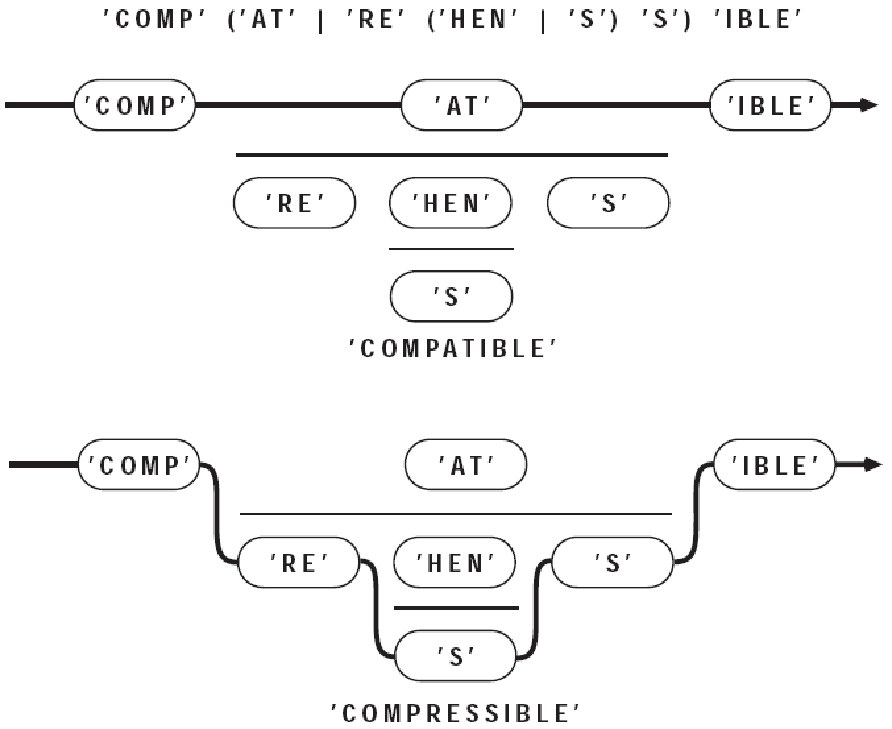
\includegraphics[width=4.9in]{beaddia.png}
\caption{Bead Diagram}
\end{figure}

Consider the following pattern and its application

\begin{verbatim}
        Manufacturer := "SONY" .| "DELL"
        Type := "Desktop" .| "Laptop"
        Machine := Manufacturer || " " || Type
        "SONY Laptop" ?? Machine
\end{verbatim}

\noindent
The pattern matching will succeed. However we would also like to
determine which of the pattern alternatives actually matched. For this
we use the conditional binary operator \(-\!\!>\). The operator is
called conditional, because assignment occurs only if the pattern
match is successful. It assigns the matching substring on its left to
the variable on its right. Note that the direction of assignment is
just the opposite of the assignment operator $:=$. Changing the above
example to use conditional assignment.

\begin{verbatim}
        Manufacturer := ("SONY" .| "DELL") -> Corporation
        Type := ("Desktop" .| "Laptop") -> SysType
        Machine := Manufacturer || " " || Type
        "SONY Laptop" ?? Machine
        write(Corporation)
        write(SysType)
OUTPUT
        SONY
        Laptop
\end{verbatim}

The immediate assignment operator \texttt{=$>$} allows us to capture
intermediate results during the pattern match. Immediate assignment
occurs whenever a subpattern matches, even if the entire pattern match
ultimately fails. Like conditional assignment, the matching substring
on its left is assigned to the variable on its right. Immediate
assignment is often used as a debugging tool to observe the pattern
matching process. When used with unevaluated expressions immediate
assignment allows creation of a powerful class of patterns as we will
see later.

During a pattern match, the cursor is Unicon's pointer into the
subject string. It is integer valued, and points between two subject
characters. It may also may be positioned before the first subject
character, or after the final subject character. Its value may never
exceed the size of the subject string by more than 1.  An example of
the index numbering system for the subject string UNICON can be found
in below, in the discussion of the function \texttt{Pos()}.

The cursor is set to 1 when a pattern match begins, corresponding to a
position immediately to the left of the first subject character. As
the pattern match proceeds, the cursor moves right and left across the
subject to indicate where Unicon is attempting a match. The value of
the cursor is assigned by the unary cursor position operator
\texttt{.$>$} to a variable. It appears within a pattern, preceding the
name of a variable. For example,

\begin{verbatim}
        p := ( "b" .| "r") || ("e" .|"ea") || ("d" .| "ds")
        pattern := .>x || p || .>y
        write("the beads are red")
        if "the beads are red" ?? pattern then 
                write(repl(" ",x - 1) , repl("_", y - x))
\end{verbatim}

The above code will underline the part of the substring that is
matched by the pattern. The output is

\begin{verbatim}
the beads are red
    -----
\end{verbatim}

Table 1 summarizes the Unicon pattern matching operators.

\begin{table}[h]
\begin{center}
	{\begin{tabular}{ | l | l | } \hline 
	Operator & Operation \\ \hline
	\textbar\textbar & Pattern concatenate \\
	\(.|\) & Pattern alternation \\
	\(-\!\!>\) & Conditional assignment \\
	$=>$ & Immediate assignment \\
	$.>$ & Cursor position assignment \\
	\hline
	\end{tabular}}
	%\newline \newline
 	\caption{Pattern Construction Operators}
	\label{Table 1: Pattern Construction Operators}
\end{center}
\end{table}

The previous examples used patterns created from literal
strings. Instead of specific characters, qualities of the string to be
matched can also be specified.The ability to specify these qualities
makes patterns powerful at recognizing more abstract patterns. There
are 3 different types of pattern construction functions that allow
specification of pattern qualities:

\begin{itemize}
\item Integer pattern functions
\item Character pattern functions
\item Pattern primitives
\end{itemize}

\subsection{Integer Pattern Functions}

These pattern construction functions take an integer as a parameter
and return a pattern as result. The integer pattern functions are:

\subsubsection{Len(i): Match fixed-length string}

{\tt Len(i)} produces a pattern which matches a string exactly i characters
long. i must be an integer greater than or equal to zero. Any
character may appear in the matched string. For example, {\tt Len(5)}
matches any 5-character string, and {\tt Len(0)} matches the empty
string. {\tt Len()} may be constrained to certain portions of the subject
by other adjacent patterns:

\begin{verbatim}
        s := "abcda"
        write(s ?? Len(3) -> out)
        s ?? Len(2) -> out || "a"
        write(out)
OUTPUT
abc
cd
\end{verbatim}

The first pattern match had only one constraint: the subject had
to be at least three characters long. Thus {\tt Len(3)} matched its first
three characters. The second case imposes the additional restriction
that {\tt Len(2)}'s match be followed immediately by the letter
{\tt "a"}. This disqualifies the intermediate match attempts
{\tt "ab"} and {\tt "bc"}.

Using {\tt Len()} with keyword {\tt \&ascii} as the subject provides a
simple way to obtain a string of unprintable characters. For example,
the ASCII control characters occupy positions 0 through 31 in the
256-character ASCII set. To obtain a 32-character string containing
these control codes, use:

\begin{verbatim}
        &ascii ?? Len(32) -> controls
\end{verbatim}

\subsubsection{Pos(i), Rpos(i): Verify cursor position}

The {\tt Pos(i)} and {\tt Rpos(i)} patterns do not match subject
characters. Instead, they succeed only if the current cursor position
is a specified value. They often are used to tie points of the pattern
to specific character positions in the subject. The following shows
the cursor positions as used by {\tt Pos()}:

\begin{figure}[h]
\centering
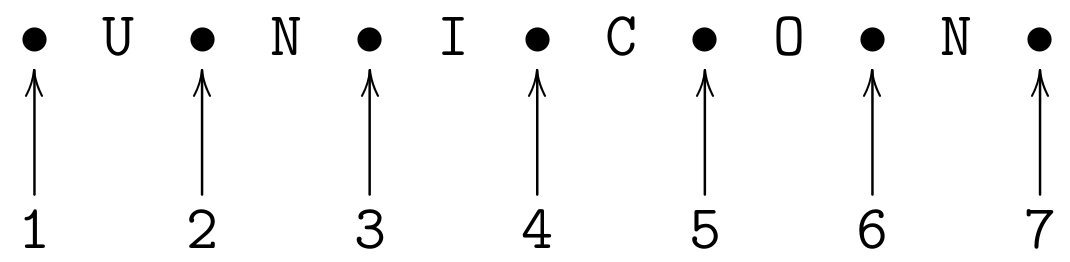
\includegraphics[width=5in]{poscurs.png}
\end{figure}

\pagebreak

The following are the cursor positions used by Rpos().

\begin{figure}[h]
\centering
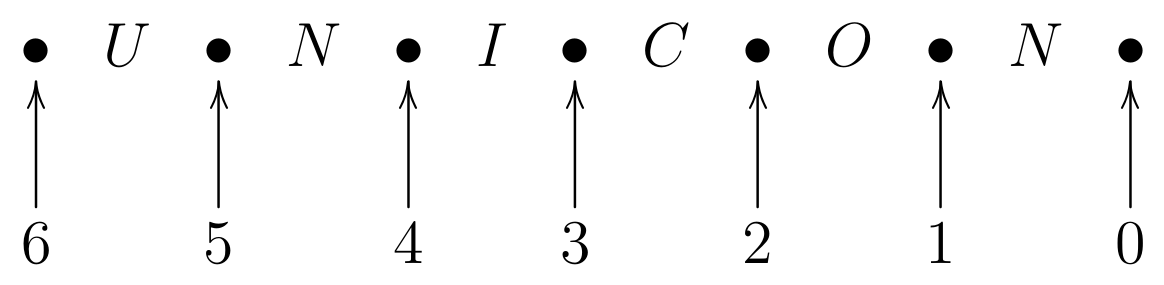
\includegraphics[width=5in]{rposcurs.png}
\end{figure}

%\begin{displaymath}
%\xymatrix@C=4pt{ \bullet & U &  \bullet & N &  \bullet & I &  \bullet & C & \bullet  & O &  \bullet & N &  \bullet \\
%	  6 \ar[u] &   & 5 \ar[u] &   & 4 \ar[u] &   & 3 \ar[u] &   & 2 \ar[u] %&   & 1 \ar[u] &   & 0 \ar[u]
%	}
%\end{displaymath}

{\tt Pos(I)} counts from the left end of the subject string, succeeding if
the current cursor position is equal to I. {\tt Rpos(I)} is similar, but
counts from the right end of the subject. If the subject length is N
characters, {\tt Rpos(I)} requires the cursor be (N - I). If the cursor is
not the correct value, these functions fail, and the pattern matcher
tries other pattern alternatives.

\begin{verbatim}
        s := "abcda"
        if s ?? Pos(1) || "b" then
                write("Match succeeded")
        else
                write("Match failed")
        s ?? Len(3) -> out || Rpos(0) 
	write(out)
        s ?? Pos(4) || Len(1) -> out
	write(out)
        if s ?? Pos(1) || "abcd" || Rpos(0) then
                write("Match succeeded")
        else
                write("Match failed")
OUTPUT
Match failed
cda
d
Match failed
\end{verbatim}

The first example requires a {\tt "b"} at cursor position 1, and fails for
this subject. {\tt Pos(1)} anchors the match, forcing it to begin with the
first subject character. Similarly, {\tt Rpos(0)} anchors the end of the
pattern to the tail of the subject. The next example matches at a
specific mid-string character position, {\tt Pos(3)}. Finally, enclosing a
pattern between {\tt Pos(1)} and {\tt Rpos(0)} forces the match to use the
entire subject string.  At first glance these functions appear to be
setting the cursor to a specified value. Actually, they never alter
the cursor, but instead wait for the cursor to come to them as various
match alternatives are attempted.

\subsubsection{Rtab(i), Tab(i): Match to fixed position}

These patterns are hybrids of {\tt Arb()}, {\tt Pos()}, and {\tt Rpos()}.
They use specific cursor positions, like {\tt Pos()} and {\tt Rpos()},
but match subject characters, like {\tt Arb()} (see section 4.4.2).
{\tt Tab(i)} matches any characters from the
current cursor position up to the specified position {\tt i}. {\tt Rtab(i)}
does the same, except, as in {\tt Rpos()}, the target position is measured
from the end of the subject.  {\tt Tab()} and {\tt Rtab()} will match the
empty string, but
will fail if the current cursor is to the right of the target. They
also fail if the target position is past the end of the subject
string.  These patterns are useful when working with tabular data. For
example, if a data file contains name, street address, city and state
in columns 1, 30, 60, and 75, this pattern will break out those
elements from a line:

\begin{verbatim}
P = Tab(30) -> NAME || Tab(60) -> STREET || 
	Tab(75) -> CITY || Rem() -> ST
\end{verbatim}

The pattern {\tt Rtab(0)} is equivalent to primitive pattern {\tt Rem()}.
It counts from the right end of the subject, but matches to the left of
its target cursor. Example:

\begin{verbatim}
        s := "abcde"
        s ?? Tab(3) -> out1 || Rtab(1) -> out2
	write(out1, "\n", out2)
OUTPUT
ab
cd
Success
\end{verbatim}


{\tt Tab(3)} matches \texttt{"ab"}, leaving the cursor at 2, between
\texttt{"b"} and \texttt{"c"}. The subject is 5 characters long, so
{\tt Rtab(1)} specifies a target cursor of 6 - 1, or 5, which is between
the {\tt "d"} and {\tt "e"}.
{\tt Rtab()} matches everything from the current cursor,
3, to the target, 5.

\subsection{Character Pattern Functions}

These functions produce a pattern based on a character set
argument. The argument passed to these functions is always converted
to a character set

\subsubsection{Any(c), NotAny(c): Match one character}

{\tt Any(c)} matches the next subject character if it appears in the cset
{\tt c}, and fails otherwise. {\tt NotAny(c)} matches a subject
character only if it does not appear in {\tt c}. Here are some sample
uses of each:

\begin{verbatim}
        vowel := Any("aeiou")
        dvowel := vowel || vowel
        notvowel := NotAny("aeiou")
        "vacuum" ?? vowel -> out
	write(out)
        "vacuum" ?? dvowel -> out
	write(out)
        "vacuum" ?? (vowel || notvowel) -> out
	write(out)
OUTPUT
a
uu
ac
\end{verbatim}

In a larger pattern context, and when many alternatives are being
tried, you may search for the multi-letter vowel combinations before
falling back on a single-letter vowel match. A pattern such as:

\begin{verbatim}
   vowel := "oy" .| "ei" .| "ie" .| Any('aieouy')
\end{verbatim}

\noindent
allows a few common digraphs in the definition of vowel.  Of course, in
a complex language such as English, the rabbit-hole is almost bottomless.


\subsubsection{Break(c), Span(c), Nspan(c): Match a run of characters}

{\tt Break(c)} and {\tt Span(c)} are multi-character versions of
{\tt NotAny()} and {\tt Any()}.  These functions
require a non-empty cset argument to specify a set of characters.
{\tt Span(c)} matches one or more subject characters from the set in {\tt c}.
{\tt Span()} must match at least one subject character, and will match
the longest subject string possible.  {\tt Nspan()} matches zero or more
subject characters from set {\tt c}; it is equivalent to
{\tt (Span(c) .\textbar "")}.

{\tt Break(c)} matches up to but not including
any character in {\tt c}. The string matched must always be followed in the
subject by a character in {\tt c}. Unlike {\tt Span()} and {\tt NotAny()},
{\tt Break()}
will match the empty string.  {\tt Break()} and {\tt Span()} are called stream
functions because each streams by a series of subject
characters. {\tt Span()} is most useful for matching a group of characters
with a common trait. For example, we can say an English word is
composed of one or more alphabetic characters, apostrophes, and
hyphens. A pattern for this is:

\begin{verbatim}
        word := Span(&letter ++ "'-")
\end{verbatim}

Some patterns that can be formed by {\tt Span()} and {\tt Break()}.
\begin{table}[h]
\begin{center}
{\begin{tabular}{ | l | l | } \hline 
        Pattern & Function \\ \hline
        a run of blanks & {\tt Span(' ')} \\ \hline
	a string of digits & {\tt Span(\&digits)} \\ \hline
	a run of letters & {\tt Span(\&lettters)} \\ \hline
	everything up to the next blank & {\tt Break(' ')} \\ \hline
	everything up to the next punctuation mark & {\tt Break(',.;:!?')} \\ \hline
\end{tabular}}
\end{center}
\end{table}

\subsubsection{Breakx(): Extended Break() function}

Like SPITBOL, Unicon provides an extended version of \texttt{Break()} called
\texttt{Breakx()}. If necessary, {\tt Breakx()} will look past the
place where it
stopped to see if a longer match is possible. It will do this if some
subsequent pattern element fails to match. The pattern matcher checks
to see if extending {\tt Breakx()} might allow the subsequent pattern
element match. If so, the operation succeeds. If not, other pattern
alternatives (if any) prior to Breakx() are attempted.  Suppose the
pattern needs to match everything before the first \texttt{"e"} in a
subject string, as with:

\begin{verbatim}
        "integers" ?? Break("e") -> out
	write(out)
OUTPUT
int
\end{verbatim}

{\tt Break()} works fine in this scenario, however if whatever comes before
the first occurrence of a two-letter pattern {\tt "er"} is to be matched,
then {\tt Breakx()} is more appropriate.

\begin{verbatim}
        "integers" ?? Breakx("e") -> out || "er"
	write(out)
OUTPUT
integ
\end{verbatim}

{\tt Breakx()} stopped at the first {\tt e} in {\tt "integer"},
and tried to match
the next pattern element, the two letters {\tt "er"}. But the next subject
characters were {\tt "eg"}, a mismatch, so {\tt Breakx()} was instructed to try
again. {\tt Breakx()} extended itself to the next {\tt "e"}, where
{\tt "er"} in the
subject matches {\tt "er"} in the pattern.  The above example illustrates
that {\tt Break(c)} will never return a string containing any characters in
c, while {\tt Breakx(c)} might, if a subsequent pattern requires it.
{\tt Breakx(c)} provides a more selective, and more efficient version of
the {\tt Arb()} pattern. For example the following construction could have
been used:

\begin{verbatim}
        "integers" ?? Arb() -> out || "er"
	write(out)
OUTPUT
integ
\end{verbatim}

\noindent
but {\tt Arb()} pokes along one character at time, matching
{\tt "i"}, {\tt "in"},
{\tt "int"}, and {\tt "inte"}, before finding the desired match,
{\tt "integ"}. In
contrast, {\tt Breakx()} gets the right answer after only two attempts:
{\tt "int"} and {\tt "integ"}. The increased efficiency is even more pronounced
with a long subject.

\subsection{Primitives}

There are eight primitives built into the Unicon pattern matching
system, of which seven have known uses. They are:

\subsubsection{Rem(): Match remainder of the subject}

{\tt Rem()} will match zero or more characters at the end of the subject
string. For example

\begin{verbatim}
       "NMSU Aggies" ?? "NMSU" || Rem() -> out
       write(out)
OUTPUT
 Aggies
\end{verbatim}

The subpattern {\tt "NMSU"} is matched at its first occurrence in the
subject. {\tt Rem()} is matched from there to the end of the subject.
If the example is changed to

\begin{verbatim}
        "NMSU Aggies" ?? "Aggies" || Rem() -> out
	write(out)
OUTPUT

\end{verbatim}

\noindent the {\tt "Aggies"} matches at the end of the string leaving an empty
remainder for {\tt Rem()}. {\tt Rem()} then matches the empty string
and the assignment to the out causes just a newline to be written to the
standard output.

The pattern components to the left of {\tt Rem()} must successfully match
some portion of the subject string. {\tt Rem()} begins after the last
character matched by the earlier pattern component and matches all
subject characters till the end of the string. There is no restriction
on the particular characters matched.

\subsubsection{Arb(): Match arbitrary characters}

{\tt Arb()} matches an arbitrary number of characters from the subject
string.  It matches the shortest possible substring, including the
empty string. The pattern components on either side of {\tt Arb()} determine
what is matched. Example:

\begin{verbatim}
        "Pragmatic Programmer" ?? "a" || Arb() -> out || "a"
	write(out)
OUTPUT
gm
        "Pragmatic Programmer" ?? "a" || Arb() -> out || "g"
	write(out)
OUTPUT

\end{verbatim}

In the first statement, the {\tt Arb()} pattern is constrained on either
side by the known patterns {\tt "a"} and {\tt "a"}.
{\tt Arb()} expands to match the
subject characters between, {\tt "gm"}. Note the smaller substring between
two occurences of {\tt "a"} is matched. In the second statement, there is
nothing between {\tt "a"} and {\tt "g"}, so {\tt Arb()} matches the empty
string. {\tt Arb()} behaves like a spring, expanding as needed to fill the
gap defined by neighboring patterns.

\subsubsection{Arbno(): Match zero or more consecutive occurences of pattern}

This function produces a pattern which will match zero or more
consecutive occurrences of the pattern specified by its
argument. {\tt Arbno()} is useful when an arbitrary number of instances of
a pattern may occur. For example, {\tt Arbno(Len(3))} matches strings of
length 0, 3, 6, 9, ... There is no restriction on the complexity of
the pattern argument.  Like the {\tt Arb()} pattern, {\tt Arbno()} tries to
match the shortest possible string. Initially, it simply matches the
empty string. If a subsequent pattern component fails to match, Unicon
backs up, and asks {\tt Arbno()} to try again. Each time {\tt Arbno()} is
retried, it supplies another instance of its argument pattern.  In
other words, {\tt Arbno(PAT)} behaves like

\begin{verbatim}
( "" | PAT | PAT PAT | PAT PAT PAT | ... )
\end{verbatim}

Also like {\tt Arb()}, {\tt Arbno()} is usually used with adjacent patterns to
draw it out. Consider the following example which tests for a list of
one or more numbers separated by commas and enclosed by parentheses.

\begin{verbatim}
        item := Span(&digits)
        list := Pos(1) || "(" || item || Arbno("," || item) ||
                ")" || Rpos(0)
        if "(12,345,6)" ?? list then
                write("Match succeeded")
        else
                write("Match failed")
        if "(12,,6)" ?? list then
                write("Match succeeded")
        else
                write("Match failed")
OUTPUT
Match succeeded
Match failed
\end{verbatim}

\texttt{Arbno()} is retried and extended till the subsequent \texttt{")"}
matches. {\tt Pos(1)} and {\tt Rpos(0)} force the pattern to be applied to the
entire subject string.

\subsubsection{Abort(): End pattern match}

The {\tt Abort()} pattern causes immediate failure of the entire pattern
match, without seeking other alternatives. Usually a match succeeds
when we find a subject sequence which satisfies the pattern. The
{\tt Abort()} pattern does the opposite: if we find a certain pattern, we
will abort the match and fail immediately.  For example suppose we are
looking for an \texttt{"a"} or \texttt{"b"}, but want to fail if
\texttt{"1"} is encountered first:

\begin{verbatim}
        if "ab1" ?? Any("ab") .| "1" || Abort() then
                write("Match succeeded")
        else
                write("Match failed")
        if "1ab" ?? Any("ab") .| "1" || Abort() then
                write("Match succeeded")
        else
                write("Match failed")
OUTPUT
Match succeeded
Match failed
\end{verbatim}

The second pattern matching expression deserves some elaboration as it
shows how the pattern matching engine works. At each cursor position
all pattern alternatives are tried. In the second pattern matching
expression after the literal {\tt "1"} matches {\tt Abort()} matches causing
the pattern to fail.  The {\tt Any()} pattern thus does not get a chance to
match the character {\tt "a"} at cursor position 2.

\subsubsection{Bal(): Match balanced string }

The {\tt Bal()} function produces a pattern that matches the shortest
non-empty string in which parentheses are balanced. A string without
parentheses is also considered to be balanced, so in the absence of
parentheses, in unanchored mode {\tt Bal()} simply matches each letter
of the string one after another. According to {\tt Bal()}
the following strings are balanced:

\begin{verbatim}
(X) Y (A!(C:D)) (AB)+(CD) 9395 (8+-9/2)
\end{verbatim}

and these are not:

\begin{verbatim}
)A+B (A*(B+) (X))
\end{verbatim}

Unlike string scanning function {\tt bal()}, pattern {\tt Bal()} is
hardwired to only look for left and right parentheses. The matching
string does not have to be a well-formed expression in the algebraic
sense; it might just as easily be a Lisp S-expression or other
parenthesis-based notation. Like {\tt Arb()}, {\tt Bal()} is often
useful when constrained by other pattern components. For example:

\begin{verbatim}
        "ab+(14-2)*c" ?? Any("+-*/") || Bal() -> out || 
                        Any("+-*/") 
OUTPUT
(14-2)
\end{verbatim}

Some additional examples of using {\tt Bal()} are presented in the
program below.  Since {\tt Bal()} happily matches spaces, these
examples discard matches that consist only of a space character.
In example 1, the pattern match applied to {\tt Bal()} is used
as a generator to drive an every loop; example 2 does the same, but
also stores the matched string into a variable for convenient
processing in a separate loop body.  Example 3 uses the pattern
from within a string scanning environment.


\begin{verbatim}
procedure main()                                                                
   s1 := "(a + b) - (c - (d*e)) + (f/g)"

   # example 1
   every write(" " ~== (s1 ?? Bal()))

   # example 2
   every (s1 ?? Bal() -> z) ~== " " do
      write("z: ", image(z))                                                    

   # example 3
   s1 ? {                                                                       
      repeat {                                                                  
         if s2 := =Bal() then write("s2: ", image(s2))                          
         else {                                                                 
            write("didn't balance at ", &pos)                                   
            move(1)                                                             
            }                                                                   
         if pos(0) then break                                                   
         }                                                                      
      }                                                                         
end
\end{verbatim}

\subsubsection{Fail(): Seek other alternatives}

The {\tt Fail()} pattern signals the failure of this portion of the pattern
match, causing the pattern matcher to backtrack and seek other
alternatives. {\tt Fail()} will also suppress a successful match, which can
be very useful when the match is being performed for its side effects,
such as immediate assignment. For example this fragment will display
the subject characters, one per line:

\begin{verbatim}
        out := &output
        subject ? Len(1) => out => Fail()
\end{verbatim}

{\tt Len(1)} matches the first subject character, and immediately assigns
it to out. {\tt Fail()} tells the pattern matcher to try again, and since
there are no other alternatives, the entire match is retried at the
next subject character. Forced failure and retries continue until the
subject is exhausted. The difference between {\tt Abort()} and {\tt Fail()}
is that {\tt Abort()} stops all pattern matching, while {\tt Fail()} tells
the system to back up and try other alternatives or other subject starting
positions.

\subsubsection{Fence(): Prevent match retries}

Pattern {\tt Fence()} matches the empty string and has no effect when the
pattern matcher is moving left to right in a pattern. However, if the
pattern matcher is backing up to try other alternatives, and
encounters {\tt Fence()}, the match fails. {\tt Fence()} can be used to
lock in an earlier success. Consider the following example: The pattern
succeeds if the first {\tt "a"} or {\tt "b"} in the subject is immediately
followed by a plus sign.

\begin{verbatim}
        "1ab+" ?? Any("ab") || Fence() || "+"
\end{verbatim}

In the example above, the pattern matcher matches the {\tt "a"} and
goes through the {\tt Fence()}, only to find that {\tt "+"} does not match the
next subject character, {\tt "b"}. The pattern matcher then tries to
backtrack, but is stopped by the {\tt Fence()} and fails.  If {\tt Fence()}
were omitted, backtracking would match {\tt Any()} to {\tt "b"}, and
then proceed
forward again to match {\tt "+"}.  If {\tt Fence()} appears as the first
component of a pattern, the pattern matcher cannot back up through it
to try another subject starting position. This allows the unanchored
pattern matching mode to simulate the anchored mode.

\subsubsection{Succeed(): Match Always}

This pattern was added to Unicon to match SNOBOL4 pattern for
pattern. The authors do not know of any meaningful use of {\tt Succeed()}.


\subsection{Unevaluated Expressions}

Consider the following pattern construction example which captures the
next {\tt i} characters after a colon:

\begin{verbatim}
        npat := ":" || Len(i) -> item
\end{verbatim}

This pattern is static in the sense that the value of {\tt i} at
time of pattern construction is captured by the pattern. Even if
\texttt{i} subsequently changes the pattern uses the original value of
\texttt{i}. One way to use the current value of \texttt{i} is to
specify the pattern each time it is used.

\begin{verbatim}
        SUBJECT ?? ":" || Len(i) -> item
\end{verbatim}

However this is not only inefficient, but also a possible maintainence
nightmare. The {\em unevaluated expression\/} facility allows us to obtain
the efficiency of static pattern construction yet use the current
value of variables. An unevaluated expression is constructed by
enclosing it in a pair of backquotes (`). So we can construct the pattern
\texttt{npat} as

\begin{verbatim}
        npat := ":" || Len(`i`) -> item
\end{verbatim}

The pattern is only constructed once, and assigned to
\texttt{npat}. \texttt{i}'s current value is ignored at this
time; the variable's name is stored in the pattern.
Later, when \texttt{npat} is used in a pattern match, the
deferred evaluation operator fetches the then current value of
\texttt{i}. Deferred evaluation may appear as the argument of the
pattern functions {\tt Any()}, {\tt Break()}, {\tt Breakx()}, {\tt Len()},
{\tt NotAny()}, {\tt Pos()}, {\tt Rpos()}, {\tt Rtab()}, {\tt Span()},
or {\tt Tab()}.

\begin{verbatim}
        pat := Tab(`i`) -> out1 || Span(`s`) -> out2
	write(out1, "\n", out2)
        sub := "123aabbcc"
        i := 5
        s := "ab"
        sub ?? pat
        i := 4
        sub ?? pat
OUTPUT
123a
abb
123
aabb
\end{verbatim}

Note that \texttt{i} and \texttt{s} were undefined when \texttt{pat}
was first constructed.

\subsubsection{Immediate Assignment}

Immediate assignment can be used as a debugging aid to view the
pattern matching process. However combined with unevaluated
expressions immediate assignments give rise to a powerful class of
patterns. In these patterns a variable that is assigned to during the
pattern matching process is used later in the very same pattern match.
Consider the following example where the first part of the subject
contains the length of the field that is to be extracted. So the
pattern first assigns the length to a variable \texttt{n} and uses
that variable as a argument to Len().

\begin{verbatim}
        fpat := Span(&digits) => n || Len(`n`) -> field        
        "12abcdefghijklmn" ?? fpat
        write(field)
OUTPUT
abcdefghijkl
\end{verbatim}

\subsubsection{Lack of Recursive Pattern Support}

At the present time, Unicon's pattern facilities do not support
the use of an unevaluated expression to achieve {\em recursive}
patterns.  For example, in SNOBOL it was possible to write a
recursion comparable to the following:

\begin{verbatim}
procedure main()
   out := &output
   p := `p` || "Z" .| "Y"
   po := p -> out
   L := ["Y", "YZZZ", "XYZ", "YZZX", "AYZZZZB"]
   every !L ?? po
end
\end{verbatim}

\noindent
On Unicon, this will result in a pattern stack overflow run-time error.


\subsubsection{Limitations due to lack of eval()}

A major difference between the SNOBOL4 and Icon families is that Icon
lacks a general facility for evaluating string contents as
expressions, the ability to introduce new code on the fly that is
available in SNOBOL. To somewhat ameliorate
this limitation, the pattern feature was augmented so that certain
operations will be evaluated during the pattern matching phase instead
of the pattern construction phase.  Unicon supports the following
language constructs in unevaluated expressions.

\begin{itemize}
\item function call
\item method call
\item variable reference
\item field reference
\end{itemize}

Note the function or method calls can only have identifiers or
constants as parameters. Expressions as parameters are not
allowed. Multiple field references of the form \texttt{x.y.z} are
not yet supported. An unevaluated function or method call is used in two
ways. The pattern matcher performs the call and if it fails, treats the
failure as if a pattern subcomponent has failed and tries to
backtrack in seach of other alternatives. However if the pattern call
succeeds then the pattern matcher can either ignore the result of the
function or use the result in the pattern matching process. To specify
that the result should be used in pattern matching the unevaluated
function call is enclosed in \texttt{` `}.  Unevaluated expressions
can also include operators for example to check if a variable is non
null

\begin{verbatim}
        `\(x)`
\end{verbatim}

\noindent binary operators can be used using the prefix notation. Only one
operator or function call can be used in an unevaluated
expression. Unicon programs that use unevaluated expressions must be
compiled with the {\texttt{"-f s"} option which enables full string invocation.

\subsection{Pattern expressions and Unicon control structure}

One of the goals while introducing pattern types in Unicon was to
ensure that it integrated well with Unicon's syntax and features such
as goal directed evaluation. Unicon’s features such as generators and
limiting generators can be used along side the pattern matching
features to write concise and readable code.
The following code changes all lines of the format \\
	\textit{year month day “unchanged portion”} \\
in the input file to \\
	\textit{month day year “unchanged portion”} \\
in the output file.

\begin{verbatim}
procedure main()
        p := Fence() || Len(4) -> yr || " " || 
                        Len(4) -> mo || " " || Len(2) -> day
        in := open("leninput", "r")
        out := open("lenoutput", "w")
        every	write(out, (line := !in) ?? 
                   p := mo || " " || day || ", " || yr || " " )
end
\end{verbatim}

The following code shows how the limiting generation control structure
can be used to obtain the nth occurrence of a pattern. In this example
the word \texttt{red} before the third occurrence of \texttt{“fish”}
will be output

\begin{verbatim}
procedure main()
   s := "One fish two fish red fish blue fish"
   wrdpat := Break(&letters) || Span(&letters) -> word
   p := wrdpat || Span(" ") || "fish"
   every (s ?? p) \ 3
   write(word)
end 
\end{verbatim}


\section{Conclusions}

The pattern matching facilities are still rough around the edges, but
nevertheless provide benefits in many text processing tasks. They
allow Unicon programmers to write more succinct and efficient code to
perform text processing.

Since the new pattern facility closely follows the implementation of
patterns in SNOBOL it also provides a path for programmers to
migrate legacy SNOBOL code to Unicon. Translating SNOBOL pattern
matching code to Unicon has been simplified because of the
nearly one to one matching between SNOBOL operators and functions and
Unicon operators and functions. The lack of an {\tt eval} function in
Unicon prevents the pattern data type from exhibiting all the power
of SNOBOL patterns.


%\bibliographystyle{abbrv}
%\bibliography{utr18}

\appendix

\section*{APPENDIX A: Language Reference}
\thispagestyle{empty}
\addcontentsline{toc}{section}{APPENDICES}

\subsection*{Regular Expressions}

Regular expressions in Unicon are pattern literals; evaluation
constructs and produces a pattern value.  Regular expressions
are enclosed in tag-like $<$ and $>$ characters, within which
the usual Unicon operator syntax does not apply and instead,
the following elements are allowed.  Unicon presently
recognizes only the classic small core set of regular
expression operators and a few common extensions.
Regular expressions are extended incompatibly in myriad tools and 
if your favorite regular expression operator is not listed here,
it is probably not in Unicon at present.


\begin{description}
\item [r] -- ordinary symbol r is a regular expression that matches r.
\item [r1 r2] -- juxtaposition of two regular expressions is a concatenation.
\item [r1 {\tt \textbar} \ r2] -- alternation of two regular expressions
	produces a regular expression that matches either r1 or r2. It
	is not a generator.
\item [r{\tt *}] -- the asterisk is a postfix operator that produces a
	regular expression that matches zero or more occurrences of r.
\item [r{\tt +}] -- the plus is a postfix operator that produces a
	regular expression that matches one or more occurrences of r.
\item [r{\tt ?}] -- the question mark is a postfix operator that produces a
	regular expression that matches zero or one occurrences of r.
\item [r{\tt \{n\}}] -- the curly braces are a postfix operator that produces a
	regular expression that matches n occurrences of r.
\item [{\tt "lit"}] -- string literals produce a regular expression that
	matches the characters of the string, with the usual escapes.
\item [{\tt 'lit'}] -- cset literals produce a regular expression that
	matches any one character of the cset, with the usual escapes.
\item [{\tt {[}chars{]}}] -- square brackets produce a regular expression that
	matches any one character of the cset, with minus interpreted
	as a range character. {\em\bf Not yet implemented: hex
	or octal escapes.}
\item [.] -- in a regular expression, the period
	matches any one character except the newline character.
\item [{\tt (}r{\tt )}] -- parentheses are used for grouping and produce a
	regular expression that matches r.
\end{description}


\subsection*{Pattern Variables}

\noindent\textbf{variable} \\
a variable in a pattern definition that may not be changed during a pattern match operation.\\
\noindent\rule{16.5cm}{0.4pt}
 
\noindent\textbf{`variable`} \\
an unevaluated variable in a pattern definition that can be changed in a pattern match operation.\\

\section*{Pattern Operators}
\noindent\textbf{pattern1 $\vert\vert$	pattern2} \hfill \textbf{pattern concatenation}\\
pattern concatenation operator produces a new pattern containing the left operand followed the right operand.\\
\noindent\rule{16.5cm}{0.4pt}

\noindent\textbf{pattern1 .$\vert$ pattern2} \hfill \textbf{pattern alternation}\\
pattern alternation operator produces a pattern containing either the left operand or the right operand.\\
\noindent\rule{16.5cm}{0.1pt}

\noindent\textbf{substring -$>$ variable} \hfill\textbf{conditional assignment}\\
assigns the substring on the left to the variable on the right if the pattern match is successful.\\
\noindent\rule{16.5cm}{0.1pt}

\noindent\textbf{result $=>$ variable} \hfill\textbf{immediate assignment}\\
assigns the immediate result on the left to a variable on the right within a pattern.\\
\noindent\rule{16.5cm}{0.1pt}

\noindent\textbf{.$>$ variable} \hfill\textbf{cursor position assignment}\\
assigns the cursor position of the string to a variable on the right within a pattern.\\
\noindent\rule{16.5cm}{0.1pt}

\noindent\textbf{string ?? pattern} \hfill\textbf{comparison operator}\\
compares the string on the left to see if there are any matches of the pattern on the right in the un-anchored mode.\\
\noindent\rule{16.5cm}{0.1pt}

\noindent\textbf{=pattern} \hfill\textbf{comparison operator}\\
compares the current string in the string scanning environment to see if there is a match of the pattern on the right in the anchored mode.\\

\textbf{\section*{Pattern Built-In Functions}}

\noindent\textbf{Abort()} \hfill\textbf{pattern cancel}\\
causes an immediate failure of the entire pattern match.\\
\noindent\rule{16.5cm}{0.1pt}

\noindent\textbf{Any(c)} \hfill\textbf{match any}\\
matches any single character contained in c appearing in the subject string.\\

\noindent\textbf{Arb()} \hfill\textbf{arbitrary pattern}\\
matches zero or more characters in the subject string.\\
\noindent\rule{16.5cm}{0.1pt}

\noindent\textbf{Arbno(p)} \hfill\textbf{repetitive arbitrary pattern}\\
matches repetitive sequences of p in the subject string.\\
\noindent\rule{16.5cm}{0.1pt}

\noindent\textbf{Bal()} \hfill\textbf{balanced parentheses}\\
matches the shortest non-null string which parentheses are balanced
in the subject string.\\
\noindent\rule{16.5cm}{0.1pt}

\noindent\textbf{Break(c)} \hfill\textbf{pattern break}\\
matches any characters in the subject string up to but not including
any of the characters in cset c.\\
\noindent\rule{16.5cm}{0.1pt}

\noindent\textbf{Breakx(c)} \hfill\textbf{extended pattern break}\\
matches any characters up to any of the subject characters in c, and
will search beyond the break position for a possible larger match.\\
\noindent\rule{16.5cm}{0.1pt}

\noindent\textbf{Fail()} \hfill\textbf{pattern back}\\
signals a failure in the current portion of the pattern match and sends
an instruction to go back and try a different alternative.\\
\noindent\rule{16.5cm}{0.1pt}

\noindent\textbf{Fence()} \hfill\textbf{pattern fence}\\
signals a failure in the current portion of the pattern match
if it is trying to backing up to try other alternatives.\\
\noindent\rule{16.5cm}{0.1pt}

\noindent\textbf{Len(i)} \hfill\textbf{match fixed-length string}\\
matches a string of a length of \texttt{i} characters in the subject string.
It fails if \texttt{i} is greater than the number of characters remaining
in the subject string.\\
\noindent\rule{16.5cm}{0.1pt}

\noindent\textbf{NotAny(c)} \hfill\textbf{match anything but}\\
matches any single character not contained in character set \texttt{c}
appearing in the subject string.\\
\noindent\rule{16.5cm}{0.1pt}

\noindent\textbf{Nspan(c)} \hfill\textbf{optional pattern span}\\
matches the longest available sequence of zero or more characters
from the subject string that are contained in \texttt{c}.  \\
\noindent\rule{16.5cm}{0.1pt}

\noindent\textbf{Pos(i)} \hfill\textbf{cursor position}\\
sets the cursor or index position of the subject string to
the position \texttt{i} according the Unicon index system shown below:
\begin{verbatim}
                   -6  -5  -4  -3  -2  -1  0
                   | U | n | i | c | o | n |
                   1   2   3   4   5   6   7
\end{verbatim}
\noindent\rule{16.5cm}{0.1pt}

\noindent\textbf{Rem()} \hfill\textbf{remainder pattern}\\
matches the remainder of the subject string.\\
\noindent\rule{16.5cm}{0.1pt}

\noindent\textbf{Span(c)} \hfill\textbf{pattern span}\\
matches one or more characters from the subject string that
are contained in \texttt{c}.  It must match at least one character.\\
\noindent\rule{16.5cm}{0.1pt}

\noindent\textbf{Succeed()} \hfill\textbf{pattern succeeds}\\
produces a pattern that, when matched, will cause the surrounding
pattern match to succeed without further scrutiny.\\
\noindent\rule{16.5cm}{0.1pt}

\noindent\textbf{Tab(n)} \hfill\textbf{pattern tab}\\
matches any characters from the current cursor or index position up to
the specified position of the subject string.  \texttt{Tab()} uses the
Unicon index system shown in \texttt{Pos()} and position \texttt{n} must
be to the right of the current position.\\
\noindent\rule{16.5cm}{0.1pt}

\noindent\textbf{Rpos(n)} \hfill\textbf{reverse cursor position}\\
sets the cursor or index position of the subject string to the
position \texttt{n} back from the end of the string, equivalent to
using Unicon's negative indices in \texttt{Pos()}.
\begin{verbatim}
                   6   5   4   3   2   1   0
                   | S | N | O | B | O | L |
\end{verbatim}
\noindent\rule{16.5cm}{0.1pt}

\noindent\textbf{Rtab(i)} \hfill\textbf{pattern reverse tab}\\
matches any characters from the current cursor or index position up to
the specified position (back from the end) of the subject string,
equivalent to using a negative index in \texttt{Tab()}.
Position \texttt{n} must be to the right of the current position.\\

\section*{APPENDIX B: Monitoring Pattern Matching}

Unicon's execution monitoring facilities have been extended to allow
the observation of pattern matching execution that is otherwise
internal to the runtime system.  Pattern matching always occurs in a
string scanning context, so the execution monitoring events related
to string scanning environments, including \texttt{E\_Snew},
\texttt{E\_Sfail}, \texttt{E\_Ssusp} and \text{E\_Sresum}, are
typically monitored as part of a tool that is monitoring pattern matches.
The pre-existing events \texttt{E\_Spos}, \texttt{E\_Assign},
\texttt{E\_Value}, and \texttt{E\_Deref} also occur as side-effects
of pattern matching evaluation.

The following new events occur during pattern creation and pattern
matching.

\vspace{0.1in}

\begin{tabular}{| c | c | c |} \hline
String Scanning Event & Event Value & Meaning \\ \hline
\texttt{E\_Pattern} & number of bytes allocated & pattern (block)
allocation \\
\texttt{E\_Pelem} & number of bytes allocated & pattern element (block)
allocation \\
\texttt{E\_PatCode} & integer & pattern element code \\ \hline
\texttt{E\_PatAttempt} & 1 = anchored & attempt to match a pattern \\
\texttt{E\_PatMatch} & string matched & pattern match succeeded \\
\texttt{E\_PatFail} & (none) &  pattern match failed \\ \hline

\texttt{E\_PelemAttempt} & integer pattern code & attempt to match an element \\
\texttt{E\_PelemMatch} & integer pattern code & element match succeeded \\
\texttt{E\_PelemFail} & integer pattern code &  element match failed \\ \hline

\texttt{E\_PatArg} & value & value being matched \\
\texttt{E\_PatVal} & value & result of deferred evaluation \\ \hline
\hline\end{tabular}



\bibliographystyle{plain}
\bibliography{utr18}

\end{document}
